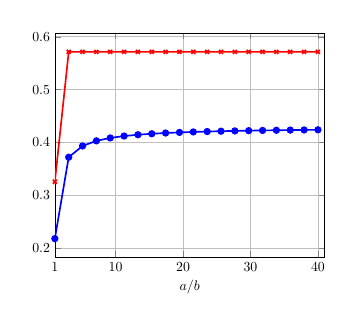
\begin{tikzpicture}[scale=0.5]
\begin{axis}[xlabel=$a/b$,ymajorgrids=true,xmajorgrids=true,xmin=1,xmax=41,xtick={1,10,20,30,40}]
%%%%%%%%%%% NATURAL CONFIGURATION
\addplot[Blue,mark=*,very thick] coordinates {(1.0,0.217751156849) (3.05263157895,0.371899923259) (5.10526315789,0.393212462993) (7.15789473684,0.402887246166) (9.21052631579,0.40840759179) (11.2631578947,0.411975544) (13.3157894737,0.414470966386) (15.3684210526,0.416314181564) (17.4210526316,0.417731290591) (19.4736842105,0.418854723411) (21.5263157895,0.419767189778) (23.5789473684,0.420523008979) (25.6315789474,0.421159327636) (27.6842105263,0.421702408465) (29.7368421053,0.422171344199) (31.7894736842,0.422580347983) (33.8421052632,0.422940218545) (35.8947368421,0.423259307375) (37.9473684211,0.423544174777) (40.0,0.423800045624) };
%%%%%%%%%%% MODIFIED CONFIGURATION
\addplot[Red,mark=x,very thick] coordinates {(1.0,0.325412497399) (3.05263157895,0.571428571428) (5.10526315789,0.571428571429) (7.15789473684,0.571428571429) (9.21052631579,0.57142857143) (11.2631578947,0.571428571429) (13.3157894737,0.571428571429) (15.3684210526,0.571428571429) (17.4210526316,0.571428571429) (19.4736842105,0.571428571429) (21.5263157895,0.571428571429) (23.5789473684,0.571428571429) (25.6315789474,0.571428571429) (27.6842105263,0.571428571429) (29.7368421053,0.571428571429) (31.7894736842,0.571428571429) (33.8421052632,0.571428571429) (35.8947368421,0.571428571429) (37.9473684211,0.571428571429) (40.0,0.571428571429) };
\end{axis}
\end{tikzpicture}
%%% Local Variables:
%%% mode: latex
%%% TeX-master: "../../mainManuscript"
%%% End:
